
%
% File divergences.tex


\documentclass[11pt,a4paper]{article}
\usepackage[draft]{hyperref}  % removing this line sometimes causes errors, but we should remove it still
\usepackage[hyperref]{naaclhlt2019}
\usepackage{times}
\usepackage{latexsym}

\usepackage{url}

%\aclfinalcopy % Uncomment this line for the final submission
\def\aclpaperid{287} %  Enter the acl Paper ID here

%\setlength\titlebox{5cm}
% You can expand the titlebox if you need extra space
% to show all the authors. Please do not make the titlebox
% smaller than 5cm (the original size); we will check this
% in the camera-ready version and ask you to change it back.

\usepackage[T1]{fontenc}
\usepackage{amsmath}
\usepackage{enumitem}
\usepackage{multirow}
\usepackage{tikz}
\usepackage{tikz-dependency}
\usepackage[warn]{textcomp}
\usepackage[font=small]{caption}
\usepackage{subcaption}
\usepackage{multirow}
\usepackage{etoolbox}
\usepackage{xr}
\usepackage{xfrac}
%\usepackage{listings}

\makeatletter
\renewcommand{\@BIBLABEL}{\@emptybiblabel}
\newcommand{\@emptybiblabel}[1]{}
\makeatother
\DeclareMathOperator*{\argmax}{arg\,max}

\newcommand{\com}[1]{}
\newcommand{\oa}[1]{\footnote{\color{red}OA: #1}}
\newcommand{\daniel}[1]{\footnote{\color{blue}DH: #1}}

\hyphenation{SemEval}
\hyphenation{English}
\hyphenation{PredPatt}


%\lstset{basicstyle=\ttfamily}


\usetikzlibrary{shapes,shapes.misc}


\title{Content Differences in Syntactic and Semantic Representations}

\author{Daniel Hershcovich$^{1,2}$ \\
  \\\And
  Omri Abend$^2$ \\
  $^1$The Edmond and Lily Safra Center for Brain Sciences \\
  $^2$School of Computer Science and Engineering \\
  Hebrew University of Jerusalem \\
  \texttt{\{danielh,oabend,arir\}@cs.huji.ac.il}
  \\\And
  Ari Rappoport$^2$
}

\date{}

\begin{document}

\maketitle

\begin{abstract}
  %1. performance gains of syntax for semantics
  %2. but, an ongoing debate
  %3. the development of "better" methods is hindered by lack of studies
  %4. we address the gap

  Syntactic analysis plays an important role in semantic parsing,
  but this role remains a topic of ongoing debate.
  The debate has been constrained by the scarcity of empirical comparative studies between syntactic and semantic schemes,
  which hinders the development of parsing methods informed by the details of target schemes and constructions.
%  as demonstrated by methods such as multi-task learning and syntactic features.
%  However, the scarcity of empirical comparative studies between syntactic and semantic schemes
  %results in existing methods being almost invariably generic,
  %  This is partly due to 
  We target this gap, and take Universal Dependencies (UD) and UCCA as a test case.
  %We emprically evaluate in what cases the two schemes converge and diverge in their content,
  After abstracting away from differences of convention or formalism,
  we find that most content divergences can be ascribed to: 
  (1) UCCA's distinction between a Scene and a non-Scene; % as opposed to UD's POS-based distinctions;
  (2) UCCA's distinction between primary relations, secondary ones and participants; %, not accounted for by UD; 
  (3) different treatment of multi-word expressions, and
  (4) different treatment of inter-clause linkage.
  We further discuss the long tail of cases where the two schemes take markedly
  different approaches.
  Finally, we show that the proposed comparison methodology can be used
  for fine-grained evaluation of UCCA parsing.
\end{abstract}


\section{Introduction}\label{sec:introduction}
  
  The promise of semantic representations stems from 
  their ability to transparently reflect distinctions relevant for text understanding
  applications. For example, syntactic representations
  are usually sensitive to distinctions based on POS (part of speech), such as between compounds
  and possessives. Semantic schemes are  less likely to make
  this distinction since a possessive can often be paraphrased as a compound
  and vice versa (e.g., ``US president''/``president of the US''),
  but may distinguish different senses of possessives (e.g., ``some of the presidents'' and ``inauguration of the presidents''),
  where a syntactic scheme would not.

  Nevertheless, little empirical study has been done on what distinguishes semantic schemes from
  syntactic ones, which are still in many cases the backbone of text understanding systems. 
  Such studies are essential for 
  (1) determining whether and to what extent semantic methods should be adopted for text understanding applications;
  (2) defining better inductive biases for parsers, and allowing better use of the information encoded in syntax;
  (3) pointing at semantic distinctions unlikely to be resolved by syntax.

  The importance of such an empirical study is emphasized by the ongoing discussion as to what role syntax should
  play in semantic parsing, if any \cite{swayamdipta2018syntactic,strubell2018linguistically,P18-1192,C18-1233}.
  See \S\ref{sec:related_work}.

  This paper aims to address this gap,
  focusing on {\it content} differences.
  As a test case, we compare relatively similar schemes (\S\ref{sec:representations}):
  the syntactic Universal Dependencies \cite[UD; ][]{nivre2016universal},
  and the semantic Universal Conceptual Cognitive Annotation \cite[UCCA; ][]{abend2013universal}.
  
  We annotate 804 UD-annotated sentences with UCCA (\S\ref{sec:shared}),
  and develop a converter to assimilate UD and UCCA,
  as they use formally different graph structures
  (\S\ref{sec:methodology}).
  We then align their nodes, and identify which UCCA categories match which UD relations,
  and which are unmatched.

  Most content differences are due to (\S\ref{sec:analysis}):
  \begin{enumerate}[noitemsep,leftmargin=*,topsep=0pt]
      \item UCCA's distinction whether a phrase evokes a Scene (event),
        as opposed to UD's POS-based distinction (predicates, nominals). % (\S\ref{sec:s}).
      \item UCCA's distinction between primary relations, secondary relations
        and Participants, as opposed to UD's core/non-core distinction. % (\S\ref{sec:arguments}).
      \item Different treatment of multi-word expressions (MWEs),
        where UCCA has a stronger tendency to identify them in the text. % (\S\ref{sec:mwe}).
      \item UCCA's conflation of several syntactic realizations of inter-clause linkage,
        and disambiguation of other cases that UD does not.
        % (e.g., infinitive vs. purposive \textit{to}). % (\S\ref{sec:linkage}).
   \end{enumerate}

  Our findings suggest that the differences between the schemes are substantial, underscoring
  the potential contribution of UCCA parsing in particular and semantic parsing in general to
  downstream text understand applications.
  For example, only 81\% of UCCA's participants are UD clausal arguments, and 84\% the other way around,
  suggesting that many semantic participants cannot be recovered from UD.\footnote{This excludes cases of shared 
  argumenthood, which are partially covered by extended UD. See \S\ref{sec:conversion}.}
  Our findings are likely to be relevant to other semantic representations, as they
  share much in terms of content \cite{abend2017state}.
    
  %   Other divergences stem from a different treatment of coordination, apposition and copulas.% (\S\ref{sec:misc}).
  
  A methodology for comparing syntactic and semantic treebanks can also support fine-grained error 
  analysis of semantic parsers, as illustrated by \citet{szubert2018structured} 
  for AMR \citep{banarescu2013abstract}.
  To demonstrate the utility of our comparison methodology,
  we perform fine-grained error analysis on UCCA parsing results
  according to UD relations (\S\ref{sec:fine_grained}).
  This analysis highlights challenges for existing UCCA parsing technology,
  and exposes cases where UCCA parsers may benefit from modeling syntactic structure more directly.


%%%%%%%%%%%%%%%%%%%%%%%%%%%%%%%%%%%%%%%%%%%%%%%%%%%%%%%%%%%%%%%%%%%%%%%%%%%%%%%%%

\section{Representations}\label{sec:representations}

  The conceptual and formal similarity between UD and UCCA can be traced back
  to their shared design principles.
  Both schemes are designed to be applicable across languages and domains, 
  to support rapid annotation and to be suitable for downstream language understanding
  applications. This section provides a brief introduction to each of the schemes, whereas
  the next sections discuss their content in further
  detail.\footnote{See Supplementary Material for a definition of each category in both schemes,
  and their abbreviations.}
  


\paragraph{UCCA}\label{sec:ucca}
%  \citep[Universal Cognitive Conceptual Annotation;][]{abend2013universal} is a
  is a semantic annotation scheme rooted in typological 
  and cognitive linguistic theory.
  It aims to represent the main semantic phenomena in text, abstracting away from syntactic forms.
  Shown to be preserved remarkably well across translations \citep{sulem2015conceptual}, it has been applied to
  improve text simplification \citep{sulem2018simple},
  and text-to-text generation evaluation \citep{birch2016hume,choshen2018usim,sulem2018samsa}.

  Formally, UCCA structures are directed acyclic graphs (DAGs) whose nodes (or {\it units}) correspond either to words,
  or to elements viewed as a single entity according to some semantic or cognitive consideration.
  Edges are labeled, indicating the role of a child in the relation the parent represents.
  A {\it Scene} is UCCA's notion of an event or a frame, and is a description of a movement, an action or a state which persists in time. 
  Every Scene contains one primary relation, which can be either a Process or a State. 
  Scenes may contain any number of Participants, a category which also includes abstract participants and locations.
  They may also contain temporal relations (Time), and secondary relations (Adverbials), 
  which cover semantic distinctions such as manner, modality and aspect.

  Scenes may be \textit{linked} to one another in several ways.
  First, a Scene can provide information about some entity,
  in which case it is marked as an Elaborator.
  This often occurs in the case of participles or relative clauses.
  For example, ``(child) who went to school'' is an Elaborator Scene
  in ``The child who went to school is John''.
  A Scene may also be a Participant in another Scene. For example, ``John went to school'' in the sentence: ``He said John went to school''. 
  In other cases, Scenes are annotated as Parallel Scenes (H), which are flat structures and may include a Linker (L), 
  as in: ``When$_L$ [he arrives]$_H$, [he will call them]$_H$''.

  Non-Scene units are headed by units of the category Center,
  denoting the type of entity or thing described by the whole unit.
  Other elements in non-Scene units include Quantifiers (such as ``{\it dozens} of people''), Connectors (mostly
  coordinating conjunctions).
  Other modifiers to the Center are marked as Elaborators.
  
%  Relators correspond in English mostly to preposition
  
  UCCA distinguishes \textit{primary} edges, corresponding 
  to explicit relations, from \textit{remote} edges,
  which allow for a unit to participate
  in several super-ordinate relations.
  See example in Figure~\ref{fig:example_ucca}.
  Primary edges form a tree, whereas remote edges (dashed) enable reentrancy, forming a DAG.
  %Table~\ref{} gives a short description of each UCCA category.  % supp. material (footnote above)

\begin{figure}[th]
  \centering
  \scalebox{.8}{
    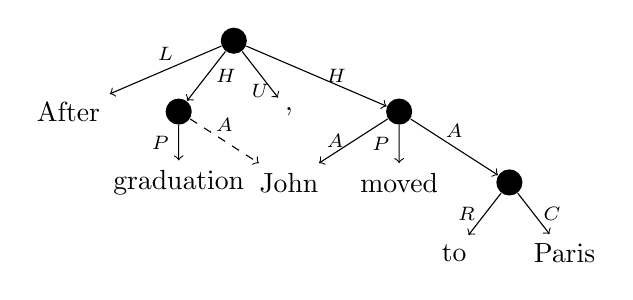
\begin{tikzpicture}[level distance=9mm, sibling distance=14mm, ->,
        every circle node/.append style={fill=black}]
      \tikzstyle{word} = [font=\rmfamily,color=black]
      \node (ROOT) [circle] {}
        child {node (After) [word] {After} edge from parent node[above] {\scriptsize $L$}}
        child {node (graduation) [circle] {}
        {
          child {node [word] {graduation} edge from parent node[left] {\scriptsize $P$}}
        } edge from parent node[right] {\scriptsize $H$} }
        child {node [word] {,} edge from parent node[below] {\scriptsize $U$}}
        child {node (moved) [circle] {}
        {
          child {node (John) [word] {John} edge from parent node[left] {\scriptsize $A$}}
          child {node [word] {moved} edge from parent node[left] {\scriptsize $P$}}
          child {node [circle] {}
          {
            child {node [word] {to} edge from parent node[left] {\scriptsize $R$}}
            child {node [word] {Paris} edge from parent node[right] {\scriptsize $C$}}
          } edge from parent node[above] {\scriptsize $A$} }
        } edge from parent node[right] {\scriptsize $H$} }
        ;
      \draw[dashed,->] (graduation) to node [above] {\scriptsize $A$} (John);
    \end{tikzpicture}
    }
\caption{\label{fig:example_ucca}
 Example UCCA graph. Dashed: a remote edge.}
\end{figure}

%%%%%%%%%%%%%%%%%%%%%%%%%%%%%%%%%%%%%%%%%%%%%%%%%%%%%%%%%%%%%%%%
\paragraph{UD}\label{sec:ud}
%\cite[UD; ][]{nivre2016universal} is
is a syntactic dependency scheme used in many languages,
aiming for cross-linguistically consistent and coarse-grained treebank
annotation. Formally, UD uses bi-lexical trees, with edge labels 
representing syntactic relations.

  One aspect of UD similar to UCCA is its preference of lexical (rather than functional) heads.
%  unlike other dependency schemes that prefer functional ones.
  For example, in auxiliary verb constructions (e.g., ``is eating''), UD
  marks the lexical verb (\textit{eating}) as the head, while other dependency schemes
  may select the auxiliary \textit{is} instead.
  While the approaches are largely inter-translatable
  \citep{Schwartz:12}, lexical head schemes are more similar in form to semantic schemes,
   such as UCCA and semantic dependencies \citep{oepen2016towards}.
%   This facilitates their comparison.
   
See example UD tree in Figure~\ref{fig:original_example_ud}.
%and Table~\ref{} gives a short description of each UD category.  % supp. material (footnote above)
UD relations are henceforth written in \texttt{typewriter} font.

\begin{figure}[th]
  \centering
    \begin{dependency}[text only label, label style={above,font=\tt}, font=\small]
    \begin{deptext}[column sep=.8em,ampersand replacement=\^]
    After \^ graduation \^ , \^ John \^ moved \^ to \^ Paris \\
    \end{deptext}
        \depedge[edge unit distance=1ex]{2}{1}{case}
        \depedge[edge unit distance=1ex]{4}{3}{punct}
        \depedge[edge unit distance=1ex]{5}{4}{nsubj}
        \depedge[edge unit distance=1ex, edge end x offset=-2pt]{2}{5}{obl}
        \depedge[edge unit distance=1ex]{7}{6}{case}
        \deproot[edge unit distance=1.5ex]{5}{root}
        \depedge[edge unit distance=1.5ex]{5}{7}{obl}
    \end{dependency}
\caption{Example UD tree.\label{fig:original_example_ud}}
\end{figure}


%%%%%%%%%%%%%%%%%%%%%%%%%%%%%%%%%%%%%%%%%%%%%%%%%%%%%%%%%%%%%%%%%%%%%%%%%%%%%%%%%%%%%%%%%%%%%%
\section{Shared Gold Standard Corpus}\label{sec:shared}

We annotate 163 English passages, containing 804 sentences
from the reviews section of the 
English Web Treebank \cite[EWT; ][]{bies2012english}.
The sentences are annotated by two UCCA annotators
according to v2.0 of the UCCA
guidelines\footnote{\tiny\url{github.com/UniversalConceptualCognitiveAnnotation/docs}}
and cross-reviewed.\footnote{The data will be released upon publication.}
As these sentences are included in the UD
English\_EWT treebank, this is a \textit{shared} gold-standard UCCA and UD
annotated corpus.

The data contains 11,103 tokens---4\% of the full UD English\_EWT treebank,
and 20\% of its reviews section.
Of the UCCA-annotated sentences, 622 belong to the UD training set,
192 to the development set and 153 to the test set.
%\daniel{Add inter-annotator agreement}


%%%%%%%%%%%%%%%%%%%%%%%%%%%%%%%%%%%%%%%%%%%%%%%%%%%%%%%%%%%%%%%%%%%%%%%%%%%%%%%%%%%%%%%%%%%%%%
\section{Comparison Methodology}\label{sec:methodology}

To facilitate comparison between UCCA and UD,
we first assimilate the graphs by abstracting away from formalism differences,
obtaining a similar graph format for both schemes.
We then match pairs of nodes in the converted UD and UCCA trees
if they share all terminals in their yields.

%One obvious difference is that
UD annotates bi-lexical dependency trees,
while UCCA graphs contain non-terminal nodes.
In \S\ref{sec:conversion}, we outline the unified DAG converter by
\citet{hershcovich2018multitask,hershcovich2018universal},\footnote{\url{http://github.com/huji-nlp/semstr}}
which we use to reach a common format.
In \S\ref{sec:local}, we describe a number of extensions
to the converter, which abstract away from further non-content differences.

\begin{figure}[th]
  \centering
  \scalebox{.8}{
  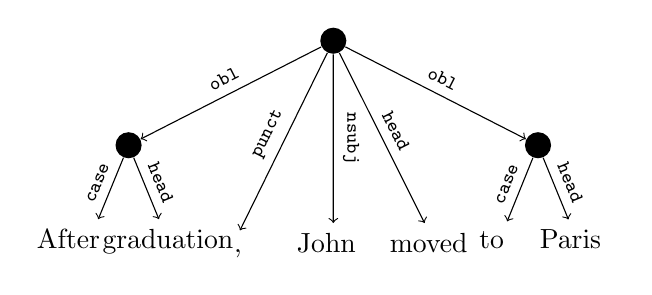
\begin{tikzpicture}[level distance=15mm, ->,
      every node/.append style={sloped,anchor=south,auto=false,font=\scriptsize\tt},
      level 1/.style={sibling distance=13mm},
      level 2/.style={sibling distance=1cm}]
    \tikzstyle{word} = [font=\rmfamily,color=black]
    \node (ROOT) [fill=black,circle] {}
      child {node (after) [fill=black,circle] {}
      {
        child {node [word] {After{\color{white}g}\quad\quad} edge from parent node {case}}
        child {node [word] {\quad graduation\quad\quad} edge from parent node {head}}
      } edge from parent node {obl}}
      child {node {}
      {
        child {node [word] (comma) {\quad,{\color{white}g}} edge from parent [draw=none]}
      } edge from parent [draw=none]}
      child {node {}
      {
        child {node [word] (John) {John{\color{white}g}} edge from parent [draw=none]}
      } edge from parent [draw=none]}
      child {node {}
      {
        child {node [word] (moved) {moved{\color{white}g}} edge from parent [draw=none]}
      } edge from parent [draw=none]}
      child {node (to) [fill=black,circle] {}
      {
          child {node [word] {to{\color{white}g}} edge from parent node {case}}
          child {node [word] {Paris{\color{white}g}} edge from parent node {head}}
      } edge from parent node {obl}}
      ;
      \draw (ROOT) to node {punct} (comma);
      \draw (ROOT) to node {nsubj} (John);
      \draw (ROOT) to node {head} (moved);
  \end{tikzpicture}}
\caption{Converted UD tree.
Intermediate non-terminals and \textit{head} edges are introduced by the unified DAG converter.
}\label{fig:converted_example_ud}
\end{figure}


\subsection{Basic Conversion}\label{sec:conversion}

Figure~\ref{fig:converted_example_ud} present the same tree from Figure~\ref{fig:original_example_ud}
after conversion.
The converter adds pre-terminals per token,
and attaches them according to the original dependency tree:
traversing it from the root, for each head it creates a non-terminal
parent with the edge label {\it head}, and adds the dependents as children of 
the created non-terminal.
Relation subtypes are stripped,
leaving only universal relations.
For example, the language-specific definite article label
\texttt{det:def} is replaced by the universal \texttt{det}.

\paragraph{Reentrancies.}
Remote edges in UCCA enable reentrancy, forming a DAG together with primary edges.
UD allows reentrancy when including \textit{enhanced dependencies}\footnote{\url{http://universaldependencies.org/u/overview/enhanced-syntax.html}}
\cite{SCHUSTER16.779}, which form (bi-lexical) graphs, representing phenomena
such as predicate ellipsis (e.g., gapping),
and shared arguments due to coordination, control, raising and relative clauses.

UCCA is more inclusive in its use of remote edges, and accounts for 
the entire class of implicit arguments termed {\it Constructional Null Instantiation} in FrameNet \citep{Ruppenhofer:16}.
For example, in
``The Pentagon is bypassing official US intelligence channels [...] in order to create strife'' (from EWT),
remote edges mark \textit{Pentagon} as a shared argument of \textit{bypassing} and
\textit{create}. 
Another example is ``if you call for an appointment [...] so you can then make one'',
where a remote edge in UCCA indicates that \textit{one} refers to \textit{appointment}.
Neither is covered by enhanced UD.

In order to facilitate comparison, we remove remote edges and enhanced dependencies in the conversion process.
We thus compare basic UD and UCCA trees, deferring a comparison of UCCA and enhanced UD to future work.



\subsection{Extensions to the Converter}\label{sec:local}

We extend the unified DAG converter to remove further non-content differences.

\paragraph{Unanalyzable units.}
Unanalyzable phrases are represented in UCCA as a single unit covering multiple terminals.
In multi-word expressions (MWEs) in UD, each word after the first is attached to the previous word,
with the \texttt{flat}, \texttt{fixed} or \texttt{goeswith} relations.
(depending on whether the expression is grammaticalized, or split by error).
We remove edges of these relations and group the corresponding terminals to one unit.
%Multi-word expressions also include compounds, discussed in \S\ref{sec:mwe}.

\paragraph{Promotion of conjunctions.}
The basic conversion generally preserves terminal yields:
the set of terminals spanned by a non-terminal is the same
as the original dependency yield of its head terminal
(e.g., in Figure~\ref{fig:converted_example_ud}, the yield of the non-terminal
headed by \textit{graduation} is ``After graduation'', the same as that of ``graduation''
in Figure~\ref{fig:original_example_ud}).

Since UD attaches subordinating and coordinating conjunctions to the following conjunct,
this results in them being positioned in the same conjunct they relate (e.g.,
\textit{After} will be included in the first conjunct in ``After arriving home, John went to sleep'';
\textit{and} will be included in the second conjunct in ``John and Mary'').
In contrast, UCCA places conjunctions as siblings to their conjuncts (e.g.,
``[After] [arriving home], [John went to sleep]'' and ``[John] [and] [Mary]''). 

To abstract away from these convention differences,
we place 
coordinating and subordinating conjunctions 
(i.e., \texttt{cc}-labeled units, and \texttt{mark}-labeled units with an \texttt{advcl} head such 
as \textit{when}, \textit{if}, \textit{after}) as siblings of their conjuncts.


%%%%%%%%%%%%%%%%%%%%%%%%%%%%%%%%%%%%%%%%%%%%%%%%%%%%%%%%%%%%%%%%%%%%%%%%%%%%%%%
\section{Analysis of Divergences}\label{sec:analysis}

Using the shared format,
we turn to discussing the content differences between UCCA and UD.


\subsection{Confusion Matrix}\label{sec:confusion}

Table~\ref{tab:confusion_matrix} presents the confusion matrix of categories between converted UD
and the UCCA, in the shared EWT corpus.
In case of multiple units with the same terminal yield (i.e., unit with a single non-remote child),
we take the top category only, to avoid double-counting.
Excluding punctuation, this results in 12,893 yields in UCCA and
13,294 in UD.
Of these, 11,541 are common, meaning that a UCCA ``parser'' developed this way
would get a very high F1 score
of 88.1\%, if given the gold UCCA label for every converted edge.

Notably, only 84\% of syntactic arguments
(\texttt{ccomp}, \texttt{csubj}, \texttt{iobj}, \texttt{nsubj}, \texttt{obj}, \texttt{obl} and \texttt{xcomp})
are Participants,
and only 81\% of Participants are syntactic arguments---a difference stemming from
the Scene/non-Scene (\S\ref{sec:s}) and argument/adjunct (\S\ref{sec:arguments}) distinctions.
%, this does not include the different treatment of shared arguments (\S\ref{sec:conversion}).

Examining the {\it head} row in Table~\ref{tab:confusion_matrix} allows
us to contrast the schemes' notions of a head. 
{\it head}-labeled units cover units that have at least
one dependent in UD, or single-clause sentences (technically, they are non-terminals added by the converter).
77.5\% correspond to Processes, States, Parallel Scenes or Centers,
which are UCCA's notions of semantic heads.
12.1\% of the {\it head} units are left unmatched, mostly due to MWEs analyzed in
UD but not in UCCA (\S\ref{sec:mwe}).
Another source of unmatched units is inter-Scene linkage, which tends to be flatter in
UCCA (\S\ref{sec:linkage}).
The rest (10.4\%) are mostly due to head swap (e.g., ``\textit{all} of Dallas'', where \textit{all}
is a Quantifier of \textit{Dallas} in UCCA, but the head in UD).

In the following subsections, we review the main content differences between the schemes,
as reflected in the confusion matrix, and categorize them according to the UD relations
involved.

\begin{table}[t]
\centering
\scriptsize
\setlength\tabcolsep{1pt}
\begin{tabular}{l|cccccccccccccc|c}
 & \bf \rotatebox{90}{Participant (A)} & \bf \rotatebox{90}{Center (C)}
 & \bf \rotatebox{90}{Adverbial (D)} & \bf \rotatebox{90}{Elaborator (E)}
 & \bf \rotatebox{90}{Function (F)} & \bf \rotatebox{90}{Ground (G)}
 & \bf \rotatebox{90}{ Parallel Scene (H)} & \bf \rotatebox{90}{Linker (L)}
 & \bf \rotatebox{90}{Connector (N)} & \bf \rotatebox{90}{Process (P)}
 & \bf \rotatebox{90}{Quantifier (Q)} & \bf \rotatebox{90}{Relator (R)}
 & \bf \rotatebox{90}{State (S)} & \bf \rotatebox{90}{Time (T)}
 & \rotatebox{90}{{\sc NoMatch}} \\
\hline
\bf \tt \tiny acl & 8 & 0 & 0 & 101 & 2 & 0 & 15 & 0 & 0 & 0 & 0 & 0 & 1 & 0 & 49 \\
\bf \tt \tiny advcl & 2 & 2 & 0 & 0 & 0 & 0 & 103 & 1 & 0 & 4 & 0 & 0 & 0 & 0 & 97 \\
\bf \tt \tiny advmod & 61 & 9 & 399 & 51 & 12 & 33 & 3 & 61 & 0 & 2 & 10 & 6 & 5 & 117 & 71 \\
\bf \tt \tiny amod & 1 & 33 & 99 & 197 & 2 & 0 & 7 & 0 & 0 & 3 & 27 & 0 & 97 & 2 & 60 \\
\bf \tt \tiny appos & 1 & 10 & 0 & 8 & 0 & 0 & 5 & 0 & 0 & 0 & 1 & 0 & 4 & 0 & 10 \\
\bf \tt \tiny aux & 0 & 0 & 96 & 0 & 285 & 0 & 0 & 0 & 0 & 0 & 0 & 0 & 0 & 0 & 2 \\
\bf \tt \tiny case & 1 & 5 & 2 & 14 & 34 & 0 & 0 & 48 & 6 & 1 & 1 & 489 & 50 & 0 & 75 \\
\bf \tt \tiny cc & 0 & 0 & 1 & 0 & 0 & 0 & 0 & 305 & 71 & 0 & 1 & 1 & 0 & 0 & 11 \\
\bf \tt \tiny ccomp & 78 & 0 & 0 & 0 & 0 & 0 & 8 & 0 & 0 & 0 & 0 & 0 & 1 & 0 & 41 \\
\bf \tt \tiny compound & 23 & 24 & 8 & 176 & 2 & 0 & 0 & 0 & 0 & 1 & 1 & 1 & 3 & 3 & 164 \\
\bf \tt \tiny conj & 2 & 88 & 1 & 0 & 0 & 0 & 265 & 0 & 0 & 2 & 0 & 0 & 3 & 0 & 90 \\
\bf \tt \tiny cop & 0 & 0 & 0 & 0 & 333 & 0 & 0 & 0 & 0 & 3 & 0 & 1 & 24 & 0 & 3 \\
\bf \tt \tiny csubj & 2 & 0 & 0 & 0 & 0 & 0 & 0 & 0 & 0 & 0 & 0 & 0 & 0 & 0 & 8 \\
\bf \tt \tiny dep & 0 & 0 & 0 & 0 & 0 & 0 & 0 & 0 & 0 & 0 & 0 & 1 & 0 & 0 & 0 \\
\bf \tt \tiny det & 2 & 1 & 19 & 763 & 1 & 1 & 0 & 0 & 0 & 0 & 19 & 2 & 0 & 0 & 26 \\
\bf \tt \tiny discourse & 0 & 1 & 0 & 0 & 1 & 6 & 13 & 3 & 0 & 0 & 0 & 0 & 1 & 0 & 1 \\
\bf \tt \tiny expl & 0 & 0 & 0 & 0 & 22 & 0 & 0 & 0 & 0 & 0 & 0 & 0 & 0 & 0 & 2 \\
\bf \tt \tiny iobj & 19 & 0 & 0 & 0 & 0 & 0 & 0 & 0 & 0 & 0 & 0 & 0 & 0 & 0 & 0 \\
\bf \tt \tiny list & 0 & 2 & 0 & 0 & 0 & 0 & 8 & 0 & 0 & 0 & 0 & 0 & 0 & 0 & 2 \\
\bf \tt \tiny mark & 0 & 2 & 3 & 0 & 186 & 1 & 0 & 134 & 1 & 0 & 0 & 53 & 1 & 1 & 18 \\
\bf \tt \tiny nmod & 100 & 1 & 1 & 233 & 0 & 0 & 6 & 0 & 0 & 0 & 0 & 0 & 3 & 4 & 110 \\
\bf \tt \tiny nsubj & 993 & 0 & 0 & 0 & 14 & 0 & 2 & 9 & 0 & 3 & 0 & 24 & 1 & 0 & 37 \\
\bf \tt \tiny nummod & 4 & 7 & 0 & 6 & 0 & 0 & 3 & 0 & 0 & 0 & 50 & 0 & 0 & 0 & 24 \\
\bf \tt \tiny obj & 439 & 7 & 5 & 1 & 1 & 0 & 1 & 1 & 0 & 8 & 1 & 6 & 0 & 4 & 92 \\
\bf \tt \tiny obl & 247 & 1 & 21 & 7 & 2 & 4 & 4 & 4 & 0 & 0 & 3 & 2 & 0 & 69 & 132 \\
\bf \tt \tiny orphan & 1 & 0 & 0 & 0 & 0 & 0 & 0 & 0 & 0 & 0 & 0 & 0 & 0 & 0 & 1 \\
\bf \tt \tiny parataxis & 1 & 0 & 0 & 1 & 0 & 2 & 79 & 0 & 0 & 1 & 0 & 0 & 2 & 0 & 39 \\
\bf \tt \tiny vocative & 9 & 0 & 0 & 0 & 0 & 3 & 0 & 0 & 0 & 0 & 0 & 0 & 0 & 0 & 0 \\
\bf \tt \tiny xcomp & 44 & 1 & 2 & 2 & 0 & 0 & 1 & 0 & 0 & 5 & 0 & 0 & 7 & 0 & 116 \\
\hline
head & 125 & 1,402 & 152 & 37 & 91 & 18 & 652 & 2 & 1 & 961 & 18 & 9 & 353 & 1 & 524 \\
\sc NoMatch & 329 & 172 & 34 & 56 & 6 & 5 & 466 & 29 & 0 & 141 & 27 & 7 & 98 & 11 & 0
\end{tabular}
\caption{UD-UCCA confusion matrix calculated from EWT
gold-standard annotations (\S\ref{sec:shared}),
after converting UD to the unified DAG format,
by comparing incoming edge labels for units with the same terminal yields.
The last column (row), labeled {\sc NoMatch}, shows the number of edges of each UD (UCCA) category
that do not match any UCCA (UD) unit.
\label{tab:confusion_matrix}}
\end{table}

\subsection{Scenes vs. Non-Scenes}\label{sec:s}

UCCA distinguishes between Scenes and non-Scenes.
This distinction crosses UD categories,
as a Scene can be evoked by a verb, an eventive or stative
noun (\textit{negotiation}, \textit{fatigue}),
an adjective or even a preposition (``this is \textit{for} John'').

\paragraph{Core syntactic arguments.}
      Subjects and objects are usually Participants (e.g., ``\textit{wine} was excellent'').
      However, when describing a Scene, such a phrase is a Process/State
      (e.g., ``But \textit{service} is very poor'').
      Some wh-pronouns are the subjects or objects of a relative clause, but
      are Linkers or Relators,
      depending on whether they link Scenes or non-Scenes, respectively.
      For example, ``who'' in ``Overall, Joe is a happy camper \textit{who} has found a great spot'' is an \texttt{nsubj}, but a Linker.

\paragraph{Adjectival modifiers} are Adverbials when modifying Scenes
    (``\textit{romantic} dinner''), States when describing non-Scenes (``\textit{beautiful} hotel'') 
    or when used predicatively (``such a \textit{convinient} location''), or
    Elaborators where defining inherent properties of non-Scenes (``\textit{medical} school'').

\paragraph{Nominal and clausal modifiers.}
    Most are Participants or Elaborators,
    depending on whether they modify a Scene (e.g.,
    ``discount \textit{on services}'' and
    ``our decision \textit{to buy when we did}'' are Participants,
    but ``\textit{my car's} gears and brakes'' and ``Some of the younger kids \textit{that work there}'' are Elaborators).
    Unmatched \texttt{acl} are often
    free relative clauses (e.g., in ``the prices were worth what \textit{I got}'',
    \textit{what} is the \texttt{obj} of \textit{worth} but
    a Participant of \textit{I got}).

\paragraph{Case markers.}
      While mostly Relators
      modifying non-Scenes (e.g., ``the team \textit{at} Bradley Chevron''),
      some are Linkers linking Scenes together 
      (e.g., ``Very informative website \textit{with} a lot of good work'').
      Others are Elaborators (e.g., ``\textit{over} a year'') or States
      when used as the main relation in verbless or copula clauses
      (e.g., ``it is right \textit{on} Wisconsin Ave'').
    
\paragraph{Coordination.}
      Coordinating conjunctions (\texttt{cc}) are Connectors where they coordinate non-Scenes
      (e.g., ``Mercedes \textit{and} Dan'')
      or Linkers where they coordinate Scenes (e.g., ``outdated \textit{but} not bad'').
      Similarly, conjuncts and list elements (\texttt{conj}, \texttt{list}) may be Parallel Scenes (H),
      or Centers when they are non-Scenes.\footnote{While in UD 
      the conjunction \texttt{cc} is attached to the following conjunct,
      in UCCA coordination is a flat structure.
      This is a convention difference that we normalize (\S\ref{sec:local}).}

\paragraph{Determiners.}
      Articles are Elaborators, and so are determiners that modify non-Scenes 
      (e.g., ``I will never recommend this gym to \textit{any} woman'').
      However, where modifying Scenes (mostly negation)
      they are marked as Adverbials. For example, ``\textit{no} feathers in stock'', ``\textit{what} a mistake'',
      and ``the rear window had \textit{some} leakage'' are all Adverbials.



\subsection{Primary and Secondary Relations}\label{sec:arguments}

UD distinguishes core arguments, adverbial modifiers,
and obliques, which in English UD correspond to prepositional dependents of a verb.
UCCA distinguishes Participants, including locations and abstract entities,
from secondary relations (Adverbials), 
which cover manner, aspect and modality.
Adverbials can be verbs (e.g., \textit{begin}, \textit{fail}),
prepositional phrases (\textit{with disrespect}),
as well as modals, adjectives and adverbs.

\paragraph{Adverbial modifiers and obliques.}
    Adverbial modifiers are mostly Adverbials (e.g., ``I \textit{sometimes} go''),
    but they may be Participants, mostly in the case of semantic arguments describing location (e.g., \textit{here}).
    Obliques
%   generally correspond in English to prepositional phrases, and
    may be
    Participants (e.g., ``wait \textit{for Nick}''), Time (e.g., ``for over 7 years'') 
    or Adverbials---mostly manner adjuncts (``by far'').

\paragraph{Clausal arguments}
    are Participant Scenes
    (e.g., ``it was great \textit{that they did not charge a service fee}'',
    ``did not really know \textit{what I wanted}'' or
    ``I asked them \textit{to change it}'').
    However, when serving as complements to a secondary verb, they
    will not match any unit in UCCA, as it places secondary verbs on the 
    same level as their primary relation. 
    For example, \textit{to pay} is an \texttt{xcomp} in ``they have to pay'', while
    the UCCA structure is flat: \textit{have to} is an Adverbial and \textit{pay} is a Process.
    Single-worded clausal arguments may correspond to a Process/State,
    as in ``this seems \textit{great}''.

\paragraph{Auxiliary verbs}
    are Functions (e.g., ``\textit{do} not forget''),
    or Adverbials when they are modals (e.g., ``you \textit{can} graduate''). Semi-modals 
    in UD are treated as clausal heads, which take a clausal complement. 
    For example, in ``able to do well'', UD treats \textit{able} as the head,
    which takes \textit{do well} as an \texttt{xcomp}. UCCA, on the other hand,
    treats it as an Adverbial, creating a mismatch for \texttt{xcomp}.
    

\subsection{Multi-Word Expressions}\label{sec:mwe}

UD and UCCA treat MWEs differently.
In UD they include names, compounds and grammaticalized fixed expressions.
UCCA treats names and grammaticalized MWEs as unanalyzable units,
but also a range of semantically opaque constructions
(e.g., light verbs and idioms).
On the other hand, compounds are not necessarily unanalyzable in UCCA,
especially if compositional.

\paragraph{Compounds.} English compounds are mostly nominal,
        and are a very heterogeneous category.
        Most compounds correspond to Elaborators (e.g., ``\textit{industry} standard''),
        or Elaborator Scenes (e.g., ``\textit{out-of-place} flat-screen TV''),
        and many are unanalyzable expressions (e.g., ``\textit{mark} up'').
        Where the head noun evokes a Scene, the dependent is often a Participant
        (e.g., ``\textit{food} craving''), but can also be an Adverbial 
        (e.g., ``\textit{first time} buyers'') depending on its semantic category.
        %In cases where t UCCA annotates both parts  may be a co-Center (e.g., ``\textit{sweet potato} tempura'').
        Other compounds in UD are phrasal verbs (e.g., ``figure \textit{out}'', ``cleaned \textit{up}''),
        which UCCA treats as unanalyzable (leading to an unmatched unit). 
            
\paragraph{Core arguments.}
      A significant number of subjects and objects are left unmatched as they
      form parts of MWEs marked in UCCA as unanalyzable. UD annotates
      MWEs involving a verb and its argument(s) just like any other clause, and therefore
      lacks this semantic content. Examples include light verbs (e.g., ``give {\it a try}''),
      idioms (``bites {\it the dust}''), and figures of speech (e.g., ``when \textit{it} comes to''),
      treated as single UCCA units.
      
\paragraph{Complex prepositions.} Some complex prepositions (e.g., \textit{according to} or \textit{on top of}),
      not encoded as MWEs in UD, are unanalyzable in UCCA.


\subsection{Linkage}\label{sec:linkage}

\paragraph{Head selection.}
UCCA tends to flatten linkage, where UD, being a dependency scheme,
has to select a head and dependent.
This yields scope ambiguities for coordination, an inherently flat structure. 
For instance, ``unique gifts and cards'' is ambiguous in UD as to whether
\textit{unique} applies only to \textit{gifts} or to the whole phrase---both
annotated as in Figure~\ref{fig:conj_ud}.
UCCA, allowing non-terminal nodes, disambiguates this case (Figure~\ref{fig:conj_ucca}).

% For camera-ready: add this to the UCCA-annotated set
% 1	unique	unique	ADJ	JJ	Degree=Pos	2	amod	_	_
% 2	gifts	gift	NOUN	NNS	Number=Plur	0	root	_	_
% 3	and	and	CCONJ	CC	_	4	cc	_	_
% 4	cards	card	NOUN	NNS	Number=Plur	2	conj	_	_

\begin{figure}[th]
  \centering
\begin{subfigure}{.45\columnwidth}
    \begin{dependency}[text only label, label style={above,font=\tt}, font=\small, edge unit distance=2ex]
    \begin{deptext}[column sep=.1em,ampersand replacement=\^]
    unique \^ gifts \^ and \^ cards \\
    \end{deptext}
        \depedge{2}{1}{amod}
        \deproot{2}{root}
        \depedge{4}{3}{cc}
        \depedge{2}{4}{conj}
    \end{dependency}
    \caption{UD.\label{fig:conj_ud}}
\end{subfigure}
\hfill
\begin{subfigure}{.45\columnwidth}
    \scalebox{.8}{
    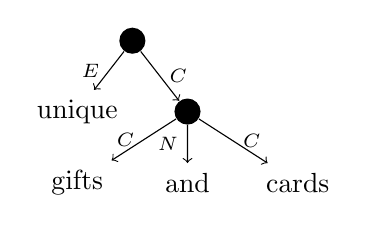
\begin{tikzpicture}[level distance=9mm, sibling distance=14mm, ->,
        every circle node/.append style={fill=black}]
      \tikzstyle{word} = [font=\rmfamily,color=black]
      \node (ROOT) [circle] {}
        child {node [word] {unique} edge from parent node[left] {\scriptsize $E$}}
        child {node [circle] {}
        {
          child {node [word] {gifts} edge from parent node[left] {\scriptsize $C$}}
          child {node [word] {and} edge from parent node[left] {\scriptsize $N$}}
          child {node [word] {cards} edge from parent node[right] {\scriptsize $C$}}
        } edge from parent node[right] {\scriptsize $C$} }
        ;
    \end{tikzpicture}
    }
    \caption{UCCA.\label{fig:conj_ucca}}
 \end{subfigure}
 \caption{Example for coordination in UD and UCCA.\label{fig:conj}}
\end{figure}


\paragraph{Clausal dependents.}
UD categorizes clause linkage into coordination,
subordination, argumenthood (complementation),
and parataxis. %(a residual category).
UCCA distinguishes argumenthood 
but conflates the other cases into Parallel Scenes,
which both adverbial clauses and parataxis
are almost exclusively marked as
(e.g., ``We called few companies before \textit{we decided to hire them}''
and ``Check out The Willow Lounge, \textit{you'll be happy}'').

Note that while in UD, \texttt{mark} (e.g., \textit{before})
is attached to the dependent adverbial clause,
a UCCA Linker lies outside the linked Scenes.
To reduce unmatched \texttt{advcl} instances,
this convention difference is fixed by the converter
(\S\ref{sec:local}).
Many remaining unmatched units are due to conjunctions we could not reliably raise.
For instance, the marker \textit{to} introducing an \texttt{xcomp} is ambiguous between Linker
(purposive \textit{to}) and Function (infinitive marker).
Similarly, wh-pronouns may be Linkers
(``he was willing to budge a little on the price {\it which} means a lot to me''),
but have other uses in questions and free relative clauses.
Other mismatches result from the long tail of differences in how UD and UCCA construe linkage.
Consider the sentence in Figure~\ref{fig:linkage}.
While \textit{moment} is an oblique argument of \textit{know} in UD,
\textit{From the moment} is analyzed as Linker in UCCA.

\begin{figure}[th]
\begin{subfigure}{\columnwidth}
  \centering
    \begin{dependency}[text only label, label style={above,font=\tt}, font=\small, edge unit distance=2ex]
    \begin{deptext}[column sep=.7em,ampersand replacement=\^]
    From \^ the \^ moment \^ you \^ enter \^ , \^ you \^ know \\
    \end{deptext}
        \depedge[edge unit distance=2.4ex]{3}{1}{case}
        \depedge{3}{2}{det}
        \depedge[edge unit distance=1ex]{8}{3}{obl}
        \depedge[edge unit distance=1.5ex]{3}{5}{acl}
        \depedge[edge unit distance=1ex]{5}{4}{nsubj}
        \depedge[edge unit distance=1.5ex]{8}{6}{punct}
        \depedge[edge start x offset=-3pt,edge unit distance=1ex]{8}{7}{nsubj}
        \deproot{8}{root}
    \end{dependency}
    \caption{UD.\label{fig:linkage_ud}}
\end{subfigure}

\begin{subfigure}{\columnwidth}
  \centering
    \scalebox{.8}{
    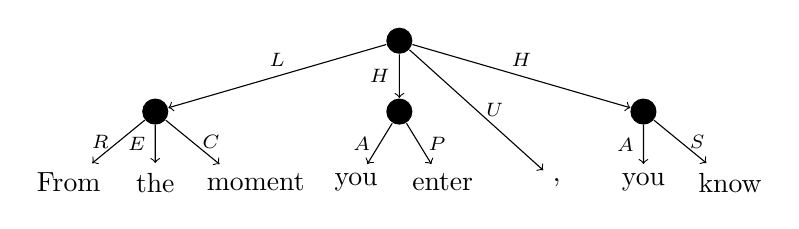
\begin{tikzpicture}[level distance=9mm, sibling distance=31mm, ->,
        level 2/.style={sibling distance=11mm},
        every circle node/.append style={fill=black}]
      \tikzstyle{word} = [font=\rmfamily,color=black]
      \node (ROOT) [circle] {}
        child {node [circle] {}
        {
          child {node [word] {From} edge from parent node[left] {\scriptsize $R$}}
          child {node [word] {the} edge from parent node[left] {\scriptsize $E$}}
          child {node [word] {\quad moment} edge from parent node[right] {\scriptsize $C$}}
        } edge from parent node[above] {\scriptsize $L$} }
        child {node [circle] {}
        {
          child {node [word] {you} edge from parent node[left] {\scriptsize $A$}}
          child {node [word] {enter} edge from parent node[right] {\scriptsize $P$}}
        } edge from parent node[left] {\scriptsize $H$} }
        child {node [circle] {}
        {
          child {node (comma) [word] {,} edge from parent [draw=none]}
          child {node [word] {you} edge from parent node[left] {\scriptsize $A$}}
          child {node [word] {know} edge from parent node[right] {\scriptsize $S$}}
        } edge from parent node[above] {\scriptsize $H$} }
        ;
      \draw[->] (ROOT) to node [right] {\scriptsize $U$} (comma);
    \end{tikzpicture}
    }
    \caption{UCCA.\label{fig:linkage_ucca}}
 \end{subfigure}
 \caption{Example for clause linkage in UD and UCCA.\label{fig:linkage}}
\end{figure}
    

\subsection{Other Differences}\label{sec:misc}

\paragraph{Appositions}
    in UD always follow the modified noun,
    but named entities in them are UCCA Centers, regardless of position
    (e.g., in ``its sister store Peking Garden'', the UD head \textit{its sister store}
    is an Elaborator, while \textit{Peking Garden} is the Center).

\paragraph{Copulas.}
    UCCA distinguishes copular constructions expressing
    identity (e.g., ``This \textit{is} the original Ham's restaurant'') where the copula is annotated as State,
    and cases of attribution 
    (e.g., ``Mercedes and Dan \textit{are} very thorough'')
    or location (e.g., ``Excellent chefs \textit{are} in the kitchen''),
    where the copula is a Function.

\paragraph{Discourse markers and interjections.}
    UCCA marks discourse markers and interjections as Ground, i.e., units that relate the Scene 
    to the speech event or to the opinion of the speaker. Examples include ``\textit{no}, Warwick in New Jersey'' and ``\textit{Please} visit my website''.
    On the other hand, discourse elements that relate one Scene to the other 
    are Linkers (e.g., ``I am sure, \textit{well}, she says'').

\paragraph{Vocatives}
    are both Ground and Participants if they participate in the Scene \textit{and} are the party addressed.
    For example, \textit{Mark} in ``Thanks \textit{Mark}'' is both the person addressed and the one thanked.\footnote{UCCA allows marking more than one category over an edge, although this
    functionality is not used often for English.}
    
\paragraph{Expletives and subjects.}
    Expletives are generally Functions,
    but some instances of \textit{it} and \textit{that} are analyzed as subjects in UD
    and as expletives in UCCA (e.g., ``\textit{it}'s like driving a new car'').    

\paragraph{Excluded relations.}
We exclude the following UD labels,
as they are irrelevant to our evaluation:
\texttt{root} (always matches the entire sentence);
\texttt{punct} (punctuation is not annotated in UCCA);
\texttt{dep} (unspecified dependency),
\texttt{orphan} (used for gapping, which is represented using remote edges in UCCA---see \S\ref{sec:conversion});
\texttt{fixed}, \texttt{flat} and \texttt{goeswith} (correspond to parts of unanalyzable units in UCCA,
    and so do not represent units on their own---see \S\ref{sec:local}).
%  \item[\texttt{clf}, \texttt{dislocated}, \texttt{reparandum}.] Not in EWT.




%\section{Improving UCCA Parsing with UD}\label{sec:silver}

%Syntactic dependency parsers require many training examples to achieve
%state-of-the-art results.
%Even after around 500K tokens, the learning curves do not seem to saturate
%\cite{de2017old,velldal2017joint}.
%
%Whereas the largest UCCA training set (English Wiki) contains 128K tokens,
%The largest joined English UD training set (EWT) contains 177K tokens.
%In French UCCA has just 10K training tokens whereas UD has 295K,
%and in German UCCA has 80K and UD 228K.
%
%\begin{table}[t]
%\centering
%\begin{tabular}{l|lll|lll}
%& \multicolumn{3}{c|}{\footnotesize \bf Primary} & \multicolumn{3}{c}{\footnotesize \bf Remote} \\
%& \footnotesize \textbf{LP} & \footnotesize \textbf{LR} & \footnotesize \textbf{LF}
%& \footnotesize \textbf{LP} & \footnotesize \textbf{LR} & \footnotesize \textbf{LF} \\
%\hline
%\footnotesize 10\% & 65.1 & 65.2 & 65.1 & 38.4 & 24.3 & 29.8\\
%\footnotesize 20\% & 68.9 & 68.3 & 68.6 & 47.1 & 28.0 & 35.2\\
%\footnotesize 30\% & 70.2 & 70.1 & 70.2 & 47.2 & 45.5 & 46.3\\
%\footnotesize 40\% & 71.5 & 71.3 & 71.4 & 52.5 & 46.1 & 49.1\\
%\footnotesize 50\% & 71.9 & 71.9 & 71.9 & 51.3 & 48.6 & 49.9\\
%\footnotesize 60\% & 71.3 & 72.4 & 71.9 & 52.9 & 45.5 & 48.9\\
%\footnotesize 70\% & 73.1 & 72.7 & 72.9 & 50.8 & 50.5 & 50.6\\
%\footnotesize 80\% & 73.5 & 72.6 & 73.0 & 52.8 & 47.0 & 49.8\\
%\footnotesize 90\% & 73.9 & 73.1 & 73.5 & 52.3 & 48.6 & 50.4\\
%\footnotesize 100\% & 74.7 & 74.8 & 74.8 & 48.5 & 51.2 & 49.8\\
%\end{tabular}
%\caption{
%Development scores for TUPA \protect\cite{hershcovich2017a} when trained on increasing amount of training data
%(English Wiki corpus).
%\label{tab:partial_data_results}}
%\end{table}
%
%Table~\ref{tab:partial_data_results} shows results for TUPA,
%trained on 10\%, 20\% etc. of the Wiki training set and tested on the Wiki development set.
%As can be seen, the primary labeled F1 continues improving substantially even from 90\% to 100\%
%of the training data. More training data is likely to yield even better performance.

\begin{table*}[th]
\centering
\scriptsize
\setlength\tabcolsep{2.1pt}
\def\arraystretch{1.5}
% \scriptsize \bf \rotatebox{90}{Primary}
\begin{tabular}{l|ccccccccccccccccccccccccccc}
& \scriptsize \bf \rotatebox{90}{\texttt{acl}}
& \scriptsize \bf \rotatebox{90}{\texttt{advcl}}
& \scriptsize \bf \rotatebox{90}{\texttt{advmod}}
& \scriptsize \bf \rotatebox{90}{\texttt{amod}}
& \scriptsize \bf \rotatebox{90}{\texttt{appos}}
& \scriptsize \bf \rotatebox{90}{\texttt{aux}}
& \scriptsize \bf \rotatebox{90}{\texttt{case}}
& \scriptsize \bf \rotatebox{90}{\texttt{cc}}
& \scriptsize \bf \rotatebox{90}{\texttt{ccomp}}
& \scriptsize \bf \rotatebox{90}{\texttt{compound}}
& \scriptsize \bf \rotatebox{90}{\texttt{conj}}
& \scriptsize \bf \rotatebox{90}{\texttt{cop}}
& \scriptsize \bf \rotatebox{90}{\texttt{csubj}}
& \scriptsize \bf \rotatebox{90}{\texttt{det}}
& \scriptsize \bf \rotatebox{90}{\texttt{discourse}}
& \scriptsize \bf \rotatebox{90}{\texttt{expl}}
& \scriptsize \bf \rotatebox{90}{\texttt{iobj}}
& \scriptsize \bf \rotatebox{90}{\texttt{list}}
& \scriptsize \bf \rotatebox{90}{\texttt{mark}}
& \scriptsize \bf \rotatebox{90}{\texttt{nmod}}
& \scriptsize \bf \rotatebox{90}{\texttt{nsubj}}
& \scriptsize \bf \rotatebox{90}{\texttt{nummod}}
& \scriptsize \bf \rotatebox{90}{\texttt{obj}}
& \scriptsize \bf \rotatebox{90}{\texttt{obl}}
& \scriptsize \bf \rotatebox{90}{\texttt{parataxis}}
& \scriptsize \bf \rotatebox{90}{\texttt{vocative}}
& \scriptsize \bf \rotatebox{90}{\texttt{xcomp}} \\
\hline
%\small \bf English EWT &  \\
\footnotesize \bf Unlabeled F1
& 53 & 49 & 91 & 90 & 63 & 97 & 92 & 93 & 59 & 79 & 75 & 98 & 29 & 96 & 96 & 88 & 81 & 67 & 96 & 82 & 94 & 81 & 73 & 65 & 55 & 50 & 56 \\
\footnotesize \bf Labeled F1
& 39 & 33 & 62 & 40 & 29 & 78 & 70 & 50 & 50 & 51 & 34 & 67 & -- & 92 & 12 & 60 & 63 & -- & 61 & 56 & 81 & 67 & 58 & 41 & 12 & 13 & 31 \\
\hline
\footnotesize \bf Total in UD & 176 & 209 & 840 & 528 & 39 & 383 & 727 & 400 & 128 & 406 & 451 & 364 & 10 & 834 & 26 & 24 & 19 & 12 & 400 & 458 & 1083 & 94 & 566 & 496 & 125 & 12 & 178 \\
\footnotesize \bf Match gold & 127 & 112 & 769 & 467 & 29 & 381 & 652 & 388 & 87 & 239 & 361 & 361 & 2 & 808 & 25 & 22 & 19 & 10 & 382 & 346 & 1046 & 70 & 474 & 364 & 86 & 12 & 62 \\
\footnotesize \bf Match pred. & 70 & 51 & 697 & 435 & 19 & 363 & 680 & 358 & 61 & 238 & 265 & 354 & 5 & 778 & 25 & 21 & 13 & 5 & 375 & 303 & 959 & 61 & 335 & 234 & 45 & 4 & 60 \\
\footnotesize \bf Unlabeled & 52 & 40 & 670 & 408 & 15 & 361 & 616 & 347 & 44 & 188 & 234 & 351 & 1 & 759 & 24 & 19 & 13 & 5 & 363 & 266 & 941 & 53 & 296 & 194 & 36 & 4 & 34 \\
\footnotesize \bf Labeled & 38 & 27 & 454 & 180 & 7 & 291 & 465 & 187 & 37 & 122 & 106 & 239 & 0 & 728 & 3 & 13 & 10 & 0 & 230 & 181 & 815 & 44 & 233 & 122 & 8 & 1 & 19 \\
\hline
\footnotesize \bf $\sfrac{\text{Labeled}}{\text{Unlabeled}}$ & 73 & 68 & 68 & 44 & 47 & 81 & 75 & 54 & 84 & 65 & 45 & 68 & 0 & 96 & 13 & 68 & 77 & 0 & 63 & 68 & 87 & 83 & 79 & 63 & 22 & 25 & 56 \\
%mode & 101 & 103 & 524 & 218 & 10 & 285 & 489 & 305 & 78 & 174 & 265 & 333 & 2 & 1 & 13 & 22 & 19 & 8 & 161 & 231 & 993 & 53 & 439 & 247 & 79 & 9 & 44 \\
\footnotesize \bf $\sfrac{\text{Mode}}{\text{Match gold}}$ & 80 & 92 & 68 & 47 & 34 & 75 & 75 & 79 & 90 & 73 & 73 & 92 & 100 & 96 & 52 & 100 & 100 & 80 & 42 & 67 & 95 & 76 & 93 & 68 & 92 & 75 & 71 \\
\footnotesize \bf $\sfrac{\text{Train Mode}}{\text{Match}}$ & 78 & 86 & 59 & 83 & 53 & 91 & 90 & 55 & 68 & 82 & 58 & 49 & 86 & 98 & 31 & 87 & 90 & 100 & 46 & 62 & 88 & 80 & 80 & 61 & 83 & 100 & 71 \\
\hline
\footnotesize \bf Mean {\#}Words & 5.1 & 6.0 & 1.2 & 1.2 & 2.9 & 1.0 & 1.0 & 1.0 & 7.4 & 1.2 & 5.3 & 1.0 & 3.3 & 1.0 & 1.0 & 1.0 & 1.1 & 2.0 & 1.0 & 2.4 & 1.6 & 1.2 & 3.1 & 3.8 & 5.7 & 1.6 & 5.8
%\small \bf English Wiki &  \\
%\small \bf English 20K &  \\
%\small \bf French 20K &  \\
%\small \bf German 20K & 
\end{tabular}
\caption{Fine-grained error analysis on the shared EWT annotated corpus.
UD relations exclude
%\texttt{clf}, \texttt{dislocated}, \texttt{reparandum},
\texttt{fixed}, \texttt{flat}, \texttt{goeswith},
\texttt{dep}, \texttt{orphan}, and \texttt{root}.
A total of 89.5\% of all UD relations matched gold-standard UCCA units
(see Table \ref{tab:confusion_matrix}).
\textit{Match gold} is the number of gold-standard UCCA units matching the UD relation units,
which is the sum of the corresponding row (without \textsc{NoMatch}) from Table~\ref{tab:confusion_matrix}.
\textit{Match pred.} is the number of matching UCCA units in the graphs predicted by TUPA.
\textit{Unlabeled} are the matched units in the intersection between the gold-standard and prediction,
where edge categories are ignored;
in \textit{Labeled} edge categories are taken into account.
\textit{Mode} refers to the number of occurrences of the most frequent gold UCCA category
to match the UD relation, according to Table~\ref{tab:confusion_matrix}
(for gold-standard UD), or in the Wiki training set that TUPA was trained on
(using UDPipe-predicted dependencies).
\textit{Mean {\#}Words} is the average number of terminals in yields corresponding to each relation
(intuitively, the more words a unit contains, the harder it is to match its terminal yield exactly).
\label{tab:fine_grained_results}}
\end{table*}

%%%%%%%%%%%%%%%%%%%%%%%%%%%%%%%%%%%%%%%%%%%%%%%%%%%%%%%%%%%%%%%%%%%%%%%%%%%%%%%%%
\section{Fine-Grained UCCA Evaluation}\label{sec:fine_grained}

In \S\ref{sec:analysis} we used our comparison methodology,
consisting of the conversion to a shared format and matching units by terminal yield,
to compare gold-standard UD and UCCA.
In this section we apply the same methodology to parser outputs,
using gold-standard UD for fine-grained evaluation.
%using both gold-standard and parsed UD for fine-grained evaluation.

\subsection{Experimental Setup}\label{sec:experiments}

%\begin{table}[t]
%\centering
%\small
%\setlength\tabcolsep{3.25pt}
%\begin{tabular}{l|ccc|ccc}
%& \multicolumn{3}{c|}{\footnotesize \bf {\#} tokens}
%& \multicolumn{3}{c}{\footnotesize \bf {\#} sentences} \\
%& \footnotesize \bf train & \footnotesize \bf dev & \footnotesize \bf test
%& \footnotesize \bf train & \footnotesize \bf dev & \footnotesize \bf test \\
%\hline
%%UCCA &&&&&&&&&&&&&&&&&& \\
%\bf English EWT &&& 11,103 &&& 804 \\
%\bf English Wiki & 124,935 & 17,784 & & 4,113 & 514 & \\
%%\bf English Wiki & 124,935 & 17,784 & 15,854 & 4,113 & 514 & 515 \\
%%Wiki 1.2.0 & 128444 & 14676 & 15313 & 4268 & 454 & 503 &&&&&&&&&&&& \\
%%\bf English 20K &&& 12,574 &&& 492 \\
%%\bf French 20K & 618 & 6,374 & 5,962 & 15 & 238 & 239 \\
%%\bf German 20K & 119,872 & 12,334 & 12,325 & 5,211 & 651 & 652
%%\multicolumn{2}{l}{20K 1.0.0/0.9.0} && 12339 &&& 506 & 10047 & 1558 & 1324 & 413 & 67 & 67 & 79894 & 10059 & 42366 & 3429 & 561 & 2164 \\
%%\hline
%%UD 2.3 & \multicolumn{2}{l}{152141} && \multicolumn{2}{l}{12543} &&
%%\multicolumn{2}{l}{250658} && \multicolumn{2}{l}{14450} && \multicolumn{2}{l}{209131} && 13814 \\
%%\hline
%\end{tabular}
%\caption{Number of tokens and sentences in the training, development and test sets
%we use for each corpus.
%% and language.
%\label{tab:corpora}}
%\end{table}

\paragraph{Data.}

In addition to the shared gold-standard English\_EWT corpus (\S\ref{sec:shared}),
we use v1.2.3 of the UCCA English Wikipedia corpus (Wiki),
with the standard train/dev/test split.
%and the \textit{Twenty Thousand Leagues Under the Sea} corpora (\textit{20K}),
%annotated in English (v1.2.2), French (v1.2.2)
%and German (v1.0.1).\footnote{\url{http://github.com/UniversalConceptualCognitiveAnnotation}}
%As in previous work, we use English 20K only as an out-of-domain test set.
%For comparability with previous work \cite{hershcovich2017a,hershcovich2018multitask},
%we also perform our experiments on Wiki v1.2.0 \cite{abend2013universal},
%on 20K v1.0.0 in English and French \cite{sulem2015conceptual},
%and on 20K v0.9.0 in German.
%For UD, we use the English\_EWT, French\_GSD and German\_GSD
%treebanks from Universal Dependencies v2.3
%\cite{11234/1-2895}.\footnote{\url{http://hdl.handle.net/11234/1-2895}}
%These are the largest freely-available UD treebanks for these languages.
For UD,
we use the English\_EWT treebank from Universal Dependencies v2.3
\cite{11234/1-2895},\footnote{\url{http://hdl.handle.net/11234/1-2895}}
filtering it to get only the 804 sentences that were also annotated in UCCA.
We additionally use UDPipe v1.2 \cite{udpipe,udpipe:2017},
trained on
English\_EWT,\footnote{\url{http://hdl.handle.net/11234/1-2898}}
to parse the Wiki corpus to UD.



%\paragraph{Evaluation of the comparison methodology.}
%
%To quantitatively assess our conversion protocol (\S\ref{sec:methodology}),
%we begin by applying it to
%the gold-standard UD trees of the English\_EWT shared sentences,
%and evaluate the \textit{unlabeled} precision, recall and F1 score
%with the gold-standard UCCA for the same sentences.
%We use standard UCCA evaluation, matching units by their terminal yields.
%%We then apply the label mapping to get fully labeled converted UCCA graphs.


\paragraph{UCCA evaluation by gold-standard UD.}

We extend the standard UCCA evaluation to perform a fine-grained division
of both gold-standard and predicted edges,
according to the relations of the UD edges they match by terminal yield
(using converted UD with our extended converter; see \S\ref{sec:local}).
This allows error analysis of UCCA parsing according to syntactic phenomena.

We train a UCCA parser,
TUPA v1.3 \cite{hershcovich2017a,hershcovich2018multitask},
on Wiki, and evaluate it on EWT
using the gold-standard UD for matched relations.
While this is an out-of-domain evaluation scenario for TUPA,
we believe it is valuable,
as the shared annotation allows accurate fine-grained
evaluation.\footnote{By default, TUPA is trained and tested using syntactic features
predicted by spaCy (\url{http://spacy.io}).
However, using UDPipe in training and gold UD in testing yielded very similar
results, so we use the default settings.}


%\paragraph{UCCA evaluation by automatically parsed UD.}
%
%To demonstrate the applicability of fine-grained analysis on UCCA data
%without gold-standard UD,
%we use UDPipe v1.2 \cite{udpipe,udpipe:2017}, trained on the UD v2.3 treebanks,
%to parse the Wiki and 20K test sets in English, French and German.
%We use the official UDPipe models trained on the English\_EWT, French\_GSD and German\_GSD
%treebanks, respectively\footnote{\url{http://hdl.handle.net/11234/1-2898}}.


%\paragraph{Baselines.}
%
%As a point of comparison, we evaluate TUPA \cite{hershcovich2017a} on the test sets,
%after training it on the UCCA training set for each language (Wiki for English,
%and 20K for French and German).
%For equal conditions,
%we train and test TUPA using features predicted by UDPipe,
%yielding slightly lower scores than previously reported using spaCy.%\footnote{\url{https://spacy.io}}

%\paragraph{Using converted UD as ``silver-standard'' data.}
%
%Using our conversion protocol (\S\ref{sec:conversion}),
%we convert the gold-standard UD graphs into UCCA.
%We use the converted UD data as ``silver-standard'' data \cite{W17-7306,N18-1104}
%and add it to the UCCA training set for training TUPA.

%\begin{table}[t]
%\centering
%\begin{tabular}{l|lll|lll}
%& \multicolumn{3}{c|}{\footnotesize \bf Primary} & \multicolumn{3}{c}{\footnotesize \bf Remote} \\
%& \footnotesize \textbf{UP} & \footnotesize \textbf{UR} & \footnotesize \textbf{UF}
%& \footnotesize \textbf{UP} & \footnotesize \textbf{UR} & \footnotesize \textbf{UF} \\
%\hline
%\multicolumn{4}{l|}{\small \bf English EWT (shared)} & \\
%\footnotesize UD 2.3
%& 82.8 & 88.4 & 85.5 & 21 & 17.8 & 19.3 \\
%\footnotesize TUPA
%& 80.8 & 77.8 & 79.3 & 10.2 & 18.6 & 13.2 \\
%\multicolumn{4}{l|}{\small \bf English Wiki test} & \\
%\footnotesize UDPipe
%& 76.7 & 81 & 78.8 & -- & -- & -- \\
%\footnotesize TUPA
%& 87.6 & 84.9 & 86.2 & 50.9 & 52.7 & 51.8 \\
%\multicolumn{4}{l|}{\small \bf English 20K} & \\
%\footnotesize UDPipe
%& 79.9 & 84.7 & 82.3 & -- & -- & -- \\
%\footnotesize TUPA
%& 83.4 & 84.4 & 83.9 & 50.8 & 24 & 32.7 \\
%\multicolumn{4}{l|}{\small \bf French 20K test} & \\
%\footnotesize UDPipe
%& 78.5 & 83.4 & 80.9 & -- & -- & -- \\
%\footnotesize TUPA
%& 72 & 72.5 & 72.2 & 21.9 & 3 & 5.3 \\
%\multicolumn{4}{l|}{\small \bf German 20K test} & \\
%\footnotesize UDPipe
%& 81.5 & 85.3 & 83.4 & -- & -- & -- \\
%\footnotesize TUPA
%& 90.8 & 89.7 & 90.2 & 69.4 & 52.6 & 59.8
%\end{tabular}
%\caption{
%Unlabeled precision, recall and F1 (in~\%) for primary and remote edges.
%UD 2.3 is the gold-standard UD after conversion to the unified DAG format,
%and other rows correspond to automatically parsed UD after conversion (UDPipe)
%or directly parsed UCCA (TUPA).
%\label{tab:conversion_results_unlabeled}}
%\end{table}

\subsection{Results}\label{sec:results}

Table~\ref{tab:fine_grained_results} displays
fine-grained evaluation by UD relations.
%Out of the total number of dependencies in the UD trees for the shared sentences,
%we can see how many relations matched any gold-standard UCCA unit (\textit{Match gold}), and
%UCCA unit predicted by TUPA (\textit{Match pred.}).
%Out of the predicted UCCA units with a correct terminal yield (\textit{Unlabeled}),
%we can also see how many were given the correct category (\textit{Labeled}).
%For comparison, $\sfrac{\text{Mode}}{\text{Match gold}}\%$ measures how ``deterministic''
%the UCCA category is in the test EWT corpus, given the UD relation,
%and $\sfrac{\text{Train Mode}}{\text{Match}}\%$ in the training Wiki corpus.
%\textit{Mean {\#}Words} indicates how long units are on average.
TUPA does best on \texttt{det}---almost always a single word with the Elaborator category.
It performs reasonably well on \texttt{nsubj} too,
but the label is correct only 87\% of the times when the yield is correct,
even though 95\% of gold \texttt{nsubj}s are Participants.
This could be explained by the distribution in the Wiki training set,
where only 88\% are Participants, suggesting that domain adaptation techniques may help.
A similar situation happens with \texttt{cc}, \texttt{conj} and \texttt{cop},
where TUPA is severely ``confused'' by the training distribution,
despite the peaked test distribution---they are mostly Linkers, Parallel Scenes
and Functions in EWT, respectively.
For \texttt{cc} and \texttt{conj} this is a Scene/non-Scene distinction,
while for \texttt{cop} it is between identity and attribution.
For \texttt{aux}, \texttt{mark} and \texttt{nummod},
it does well despite the varied test distribution,
possibly by learning to lexically distinguish,
e.g., between modals (Adverbials) and auxiliaries (Functions),
though they are both \texttt{aux}.

TUPA does worst on \texttt{discourse}, \texttt{vocative} and \texttt{appos},
but these relations are rare,
and so would not contribute much to the overall parser score.
Several types of inter-clause linkage, which TUPA also struggles with,
are quite common: \texttt{parataxis}, \texttt{xcomp}, \texttt{advcl},
\texttt{conj} and \texttt{ccomp}.
Although the matching beteween UCCA and UD is not perfect in these cases,
it is overall better than TUPA's unlabeled performance.
The same pattern recurs when using gold standard syntax as features for TUPA.
TUPA is a transition-based parser, which uses UD parses as features. Our
results, however, suggest that encoding syntax more directly, perhaps through syntactic
scaffolding \citep{swayamdipta2018syntactic}, could assist in predicting the unit's boundaries.

In other cases, TUPA fails to disambiguate cases which are not disambiguated
in UD. For example, TUPA does poorly on distinguishing between \texttt{nmod}s that modify
scene-evoking nouns (Participants) and those modifying other nouns (Elaborators). 
This information is not to be found in UD (selecting the mode in these cases obtains
roughly the same performance as TUPA).
Relying on lexical resources that distinguish eventive and relational nouns from concrete 
nouns could help in this case, and lexical resources for light verbs and idioms could
help performance in the similar case of \texttt{compound}s.
%and similarly for \texttt{cc}, \texttt{conj}, \texttt{amod} and \texttt{obl}).


%%%%%%%%%%%%%%%%%%%%%%%%%%%%%%%%%%%%%%%%%%%%%%%%%%%%%%%%%%%%%%%%%%%%%%%%%%%%%%%%%
\section{Related Work}\label{sec:related_work}

The use of syntactic parsing as a proxy for semantic structure has a long tradition in NLP.
Indeed, semantic parsers have leveraged syntax
for output space pruning \cite{xue2004calibrating}, 
syntactic features \cite{gildea2002automatic,N15-1007,E17-1045}, 
joint modeling \cite{surdeanu2008conll,hajivc2009conll}, and
multi-task learning \cite{swayamdipta2016greedy,swayamdipta2018syntactic,strubell2018linguistically}.
Some syntactic representation approaches, notably CCG \cite{Steedman:00},
directly reflect the underlying semantics, and have been used to
transduce semantic forms using rule-based systems \cite{Basile:12}.

%Two CoNLL shared tasks on joint syntactic and semantic dependency parsing

%explored the connection between syntactic dependencies and
%semantic annotations built on top of them.
%Other works have contested the importance of syntax to semantics,
%by achieving strong performance without explicitly modeling syntax \cite{Peng-EtAl:2018:NAACL,P18-2077,P18-1192,C18-1233}.
  
However, only few works have attempted an empirical study of
the differences between syntactic and semantic schemes. 
\newcite{zhang2017evaluation} evaluated PredPatt \citep{white2016universal},
a framework for extracting predicate-argument structures from UD,
on a large set of high-quality annotations converted from PropBank.
%They evaluated the extracted predicate-argument relations using both
%gold-standard and parsed UD.
\newcite{szubert2018structured} proposed a method for aligning AMR
\cite{banarescu2013abstract} and UD subgraphs,
finding that 97\% of AMR edges are evoked by words or syntactic relations.
\newcite{damonte-17} suggested refining AMR evaluation by UD labels.
Similarly, our conversion protocol allows fine-grained evaluation of UCCA parsing.

A related line of work tackles the transduction of syntactic structures into semantic ones.
\newcite{reddy2016transforming} proposed rule-based a method for converting UD
to logical forms. 
%They map syntactic dependency relations directly to logical relations,
%assuming the predicate-argument structure is isomorphic to the dependency structure,
%but handling exceptions by rules relating to specific linguistic constructions,
%namely prepositional phrases, conjunction, relatives clauses, and wh-questions.
\newcite{stanovsky2016getting} converted Stanford Dependencies trees into
proposition structures ({\sc PropS}), abstracting away from some syntactic detail.
% to achieve a more semantically-oriented representation.


\section{Conclusion}\label{sec:conclusion}

We evaluate the similarities and divergences in the content encoded by UD and UCCA. 
We have annotated 804 sentences from the English Web Treebank corpus with gold-standard UCCA,
and used an automated methodology to evaluate how well the two schemes align, developing
a converter to abstract away from superficial structural
differences. Our findings provide a detailed picture of the content differences between the schemes, placing most of them
in one of four major categories. We further demonstrate that the comparison methodology can be used for fine-grained
evaluation of UCCA parsers, and find concrete paths for advancement in UCCA parsing, either by relying more directly on 
information already encoded by UD, or by relying on other existing resources for information not encoded in UD.\oa{this needs to turn into more exciting}

%Future work will extend our conversion protocol to a full labeled conversion,
%using .
%The converter can be used as a UCCA parser, or for generating extra training data for TUPA.

%%%%% Acknowledgments %%%%
% Jakob Prange, Nathan Schneider


\bibliography{references}
\bibliographystyle{acl_natbib}

\end{document}
